\begin{frame}
\frametitle{Contexte (2)}
\begin{center}
  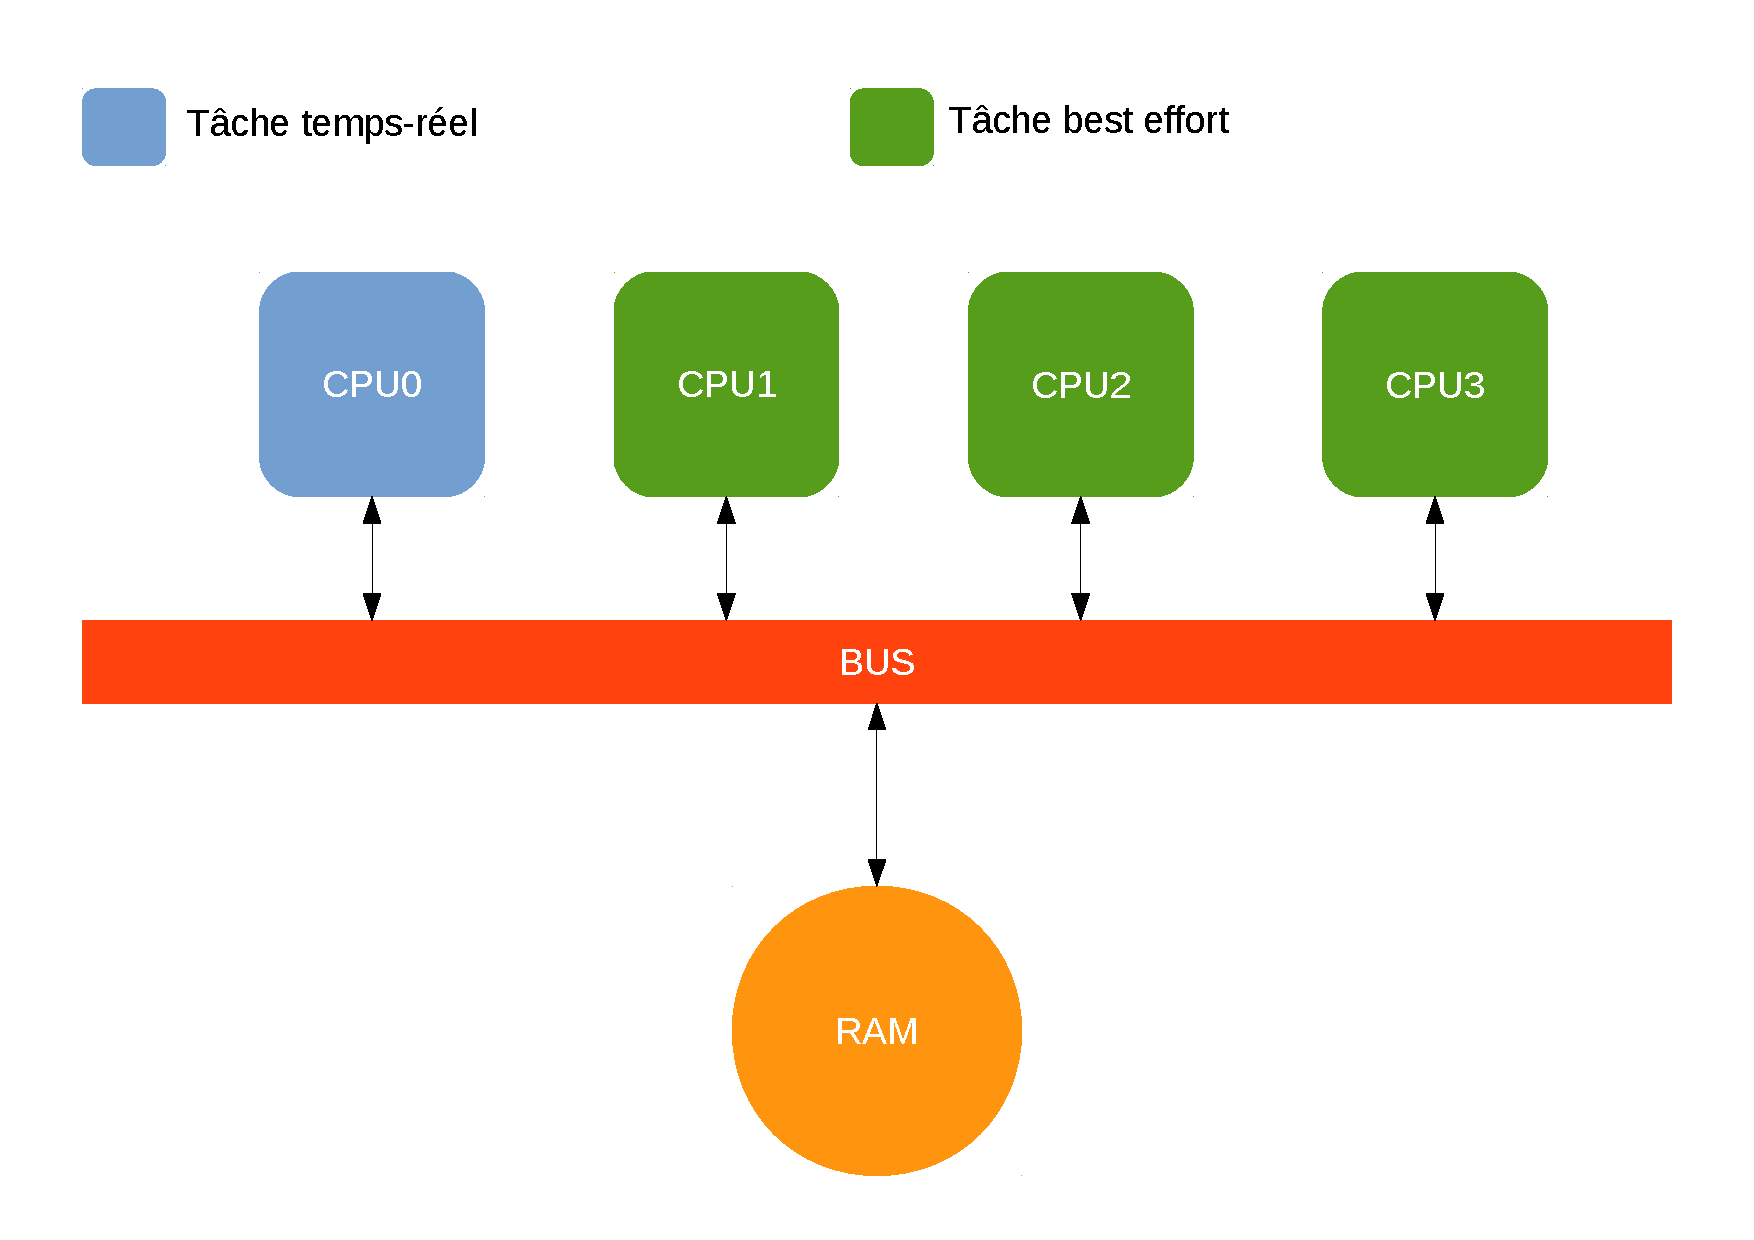
\includegraphics[scale=0.3]{include/archi.pdf}
\end{center}
\end{frame}

\begin{frame}
\frametitle{Objectifs}
\begin{itemize}
  \item Choix de l'application
  \item Parallèlisation de l'application
  \item Profilage
\end{itemize}
\end{frame}

\begin{frame}
\frametitle{Choix de l'application}
\begin{itemize}
  \item Beaucoup d'accès mémoire
  \item Trouvable dans une voiture
\end{itemize}
\end{frame}

\begin{frame}
\frametitle{Critères de selection}
\begin{itemize}
  \item Langage
  \item Nombre de dépendences
  \item Consommation mémoire
  \item Parallélisable
\end{itemize}
\end{frame}


\begin{frame}
\frametitle{Open Street Routing Machine}
Inconvénients :
\begin{itemize}
\item Nombre de dépendences élevé
\item Consommation mémoire trop élevé
\end{itemize}
\end{frame}


\begin{frame}
\frametitle{Routino}
\begin{itemize}
\item Aucune dépendence
\item Peu gourmand en mémoire
\item ... mais pas parallèle
\end{itemize}
\end{frame}



\begin{frame}
\frametitle{Algorithme de Routino}
\begin{itemize}
  \item ksjds
\end{itemize}
\end{frame}
